% Full-paper skeleton for ACM SIGMETRICS 2027 (winter cycle; POMACS format).
% Build:  latexmk -pdf main.tex   (needs TeX Live with acmart >= 2.x; not available on the
% build machine used for the research runs, so this file has not yet been compiled).
% Every number below is copied from results/*.csv; `scripts/build_workshop_battery.py`
% is the content source. Keep the two in sync until the numbers are macro-generated.
\documentclass[acmsmall,review,anonymous]{acmart}
\usepackage{amsmath,amssymb,amsthm}
\usepackage{booktabs}

\newtheorem{theorem}{Theorem}
\newtheorem{proposition}[theorem]{Proposition}
\newtheorem{lemma}[theorem]{Lemma}
\theoremstyle{definition}
\newtheorem{definition}[theorem]{Definition}

\newcommand{\Mp}{\mathcal{M}}
\newcommand{\sinc}{\operatorname{sinc}}

\setcopyright{none}
\acmJournal{POMACS}

\title{Your Data Centre Is Already a Battery: A Closed-Form Theory of Carbon-Aware Shifting under Power Caps}
\author{Anonymous Author(s)}
\affiliation{\institution{Submission for double-blind review}\country{}}

\begin{abstract}
Upper bounds on carbon-aware workload shifting assume a data centre can draw any power in
any hour. Achieving them needs the median facility to draw 13$\times$ its mean power in a single
hour. We show that the capped problem has a closed-form structure. With 24\,h slack, flexible
work water-fills each day's cleanest hours; the share of the ideal saving kept depends only on
headroom per unit of flexible load ($h/\varphi$, an exact homogeneity theorem), and the saving is
$\varphi A \sinc(\pi\varphi/(\varphi+h))$ for daily swing $A$ ($R^2=0.968$ over 4{,}680 LP solves).
More generally, flexible load under a power cap \emph{is} a lossless battery of energy
$s\varphi$, discharge power $\varphi$ and charge power $h$. This one picture explains why a UPS is
negligible, why tight caps plan beyond the slack, and why power caps stop uncoordinated
carbon-aware fleets from herding. It also marks the boundary of the theory: convex knobs
(DVFS, GPU power limits) are \emph{not} batteries. Their saving is the gap between the
arithmetic and a power mean of the carbon signal, second order in its variation:
0.79\% against 14.6\% for deferral on 123 grid zones.
\end{abstract}

\keywords{carbon-aware computing, workload shifting, power capping, virtual storage, water-filling}

\begin{document}
\maketitle

\section{Introduction}
% Source: build_workshop_battery.py §1; F3, F4, F12.
% Contributions: (1) homogeneity theorem and water-filling closed form (Thm 1, Prop 2);
% (2) virtual-battery equivalence (Thm 3) and its corollaries (UPS, horizon, signal blending);
% (3) storage exchange rate (F23); (4) the power-cap as an anti-herding device (F24);
% (5) the boundary: power-mean law for convex knobs (Thm 4, F29).
\textbf{Shifting is capped in practice.} Carbon-aware schedulers defer flexible work to hours
when the grid is cleaner~\cite{radovanovic2021carbonaware,wiesner2021lets,sukprasert2024on}.
Upper-bound studies assume the facility can absorb any amount of shifted
work~\cite{sukprasert2024on}. Achieving those bounds needs the median grid zone to draw
13$\times$ its mean power in a single hour (24\,h slack; 85$\times$ with a week). Real facilities
cannot: transformers, switchgear and UPS modules are sized for a peak. Google's released power
traces~\cite{sakalkar2019data} put the median power domain at 70\% of its rating, about +42\%
headroom, which keeps a median 54\% (44--75\%) of the ideal saving. With the cap in the model,
the remaining saving, the value of extra capacity and the right planning horizon are usually
obtained by solving a year-long linear program for every grid and parameter.

\textbf{This paper replaces those solves with a theory.} Its core is an exact equivalence:
\emph{a power-capped flexible workload is a lossless battery}. Power engineers already treat
aggregations of flexible loads as virtual storage~\cite{callaway2011achieving,hao2015aggregate};
we make the mapping exact for deferrable compute under a facility cap, solve the resulting problem
in closed form (water-filling~\cite{cover2006elements}), and test every law against the optimiser
on Electricity Maps traces for 123 grid zones over three years~\cite{maps2022hourly}.

\textbf{Contributions.}
\begin{itemize}
\item The virtual-battery theorem: energy $s\varphi$, discharge power $\varphi$, charge power $h$,
  100\% efficiency (Theorem~\ref{thm:battery}, \S\ref{sec:battery}).
\item Closed forms for the saving, the share kept, the value of a kilowatt and the peak draw, from
  water-filling and an exact homogeneity theorem (\S\ref{sec:waterfill}).
\item Three earlier empirical puzzles explained, one confirmed as a prediction: why a UPS barely
  helps, why tight caps plan beyond the slack, and why signals blend for load but not for storage.
\item A storage exchange rate: with +20\% headroom a half-flexible facility is worth a median
  4.3\,kWh of 4\,h Li-ion storage per kW of load, at 1/31 of the embodied carbon.
\item The boundary of the theory: convex knobs (DVFS, GPU power limits) are not batteries; their
  saving is a power-mean gap, second order in the signal's variation
  (Theorem~\ref{thm:powermean}; median 0.79\% against 14.6\% for deferral).
\end{itemize}

\section{Model}
\label{sec:model}
A facility has mean load $1$, hourly carbon intensity $c_t$ ($t=1,\dots,T$), a share
$\varphi\in(0,1]$ of the load that arrives as flexible work at rate $\varphi$ per hour and must be
served within $s$ hours, and a power cap $1+h$ ($h\ge0$ is the headroom). The inflexible load
$1-\varphi$ runs on arrival. Let $y_t\ge0$ be flexible work served in hour $t$,
$Y_t=\sum_{\tau\le t}y_\tau$ and $A_t=\varphi t$. Work is fluid and served earliest-deadline-first,
so the schedule is feasible iff
\begin{equation}
A_{t-s}\le Y_t\le A_t,\qquad 0\le y_t\le \varphi+h\qquad\forall t, \label{eq:lp}
\end{equation}
and the problem is $\min\sum_t c_t\,(1-\varphi+y_t)$ subject to \eqref{eq:lp}.
The saving $S(\varphi,h)$ is the drop against $y_t=\varphi$.

\section{Water-Filling and Homogeneity}
\label{sec:waterfill}
\begin{theorem}[Homogeneity]\label{thm:homog}
$S(\lambda\varphi,\lambda h)=\lambda S(\varphi,h)$ for all $\lambda>0$. Hence the share of the
ideal saving kept under a cap, $S(\varphi,h)/S(\varphi,\infty)$, is a function of $h/\varphi$ alone.
\end{theorem}
\begin{proposition}[Sinusoidal closed form]\label{prop:sinc}
With $s=24$, one-day windows and $c_t=\bar c-A\cos(2\pi t/24)$, the optimum serves the
flexible work at rate $\varphi+h$ during the cleanest fraction $q=\varphi/(\varphi+h)$ of the day and
\[ S(\varphi,h)=\varphi A\,\sinc(\pi q),\qquad \sinc x=\sin x/x. \]
The uncapped saving is $\varphi A$ and the peak draw is $1+24\varphi$.
\end{proposition}
% Empirics: uncapped R^2 0.998 (phi*A), capped R^2 0.968 (4,680 LP solves); water-level
% shadow price R^2 0.981 (results/waterfill_*.csv).

\section{Flexible Load under a Cap Is a Battery}
\label{sec:battery}
\begin{theorem}[Virtual battery]\label{thm:battery}
Let $B_t=A_t-Y_t$ (the backlog). Constraints \eqref{eq:lp} are equivalent to
\[ 0\le B_t\le s\varphi,\qquad -h\le B_t-B_{t-1}\le\varphi, \]
and the facility draws $1-(B_t-B_{t-1})$. Capped shifting is therefore exactly the dispatch of a
lossless battery of energy $s\varphi$, discharge power $\varphi$ and charge power $h$ in front of a
flat load of $1$, with boundary condition $B_0=0$, $B_T=0$ (instead of a cyclic one).
\end{theorem}
% Corollaries (F22): UPS = 1/72 of the virtual energy; effective horizon s*phi/h; lossless
% battery blends signals harmlessly in all 48 BAs; exchange rate vs a 4 h Li-ion battery (F23).

\section{Fleets: Saturation and Herding}
\label{sec:fleets}
The truly free resource for flexible load is curtailed renewable energy, and it is finite. On
CAISO 2021--2024, with curtailed energy free and a constant gas margin otherwise, the saving per
flexible kWh of a coordinated fleet falls by two-thirds between 0.1 and 1\,GW of mean load and
reaches zero near 8\,GW. A herd of independent schedulers that all follow the same exogenous signal
raises emissions from 0.5--1\,GW upwards when uncapped. With a +20--50\% power cap the herd keeps
97--100\% of the coordinated optimum: in a fleet, the cap of Section~\ref{sec:model} acts as an
anti-herding device.
% Numbers: results/curtailment_*.csv (F24).

\section{Two Batteries on One Grid}
\label{sec:twobatteries}
Theorem~\ref{thm:battery} has a consequence for grids that already have batteries: there
are then two batteries competing for the same clean surplus. Let the grid's storage fleet have
round-trip efficiency $\eta<1$ and be dispatched to minimise emissions, and let $m_t$ be the
marginal emission rate (the dual of the energy balance in hour $t$).
\begin{theorem}[No-arbitrage]\label{thm:noarb}
If in an optimal dispatch the storage fleet charges in hour $a$ and discharges in hour $b$
(after $a$, the same cycle), and neither its power limits in $a$ and $b$ nor its energy limit
between them binds, then $m_a=\eta\,m_b$. Moving one unit of flexible load from $b$ to $a$
then changes emissions by $-(1-\eta)\,m_b$ to first order.
\end{theorem}
Thus on a storage-rich grid the carbon value of shifting is the grid battery's round-trip loss,
not the hourly swing. The flexible workload is a \emph{lossless} battery
(Theorem~\ref{thm:battery}), so it still beats the grid's battery by exactly $1-\eta$, but its
value has moved from carbon to avoided storage.

\emph{Evidence (CAISO).} We add emission-minimising storage ($\eta=0.85$) on top of the
fleet already behind the observed curtailment, re-optimised in both the flat and the shifted
case ($\varphi=0.5$, cap $1/0.70$, 24\,h slack). California's 2025 battery build alone
(+4.7\,GW / 16.5\,GWh) leaves 41\% (0.1\,GW fleet) and 45\% (1\,GW fleet) of the 2024
saving, and 24--47\% over 2021--2024. With unlimited storage the saving kept is
$(1-\eta)+0.035$ or less for $\eta\in[0.7,1]$ (Figure~\ref{fig:twobatteries}). A
timing-free greedy estimate that needs no LP agrees within 5\% in 2024.
Prior work notes that storage and other flexibility cannibalise each
other~\cite{prol2021the}, that storage can raise emissions~\cite{hittinger2015bulk}, and that
demand response shrinks a data centre's battery~\cite{acun2023carbon}; we state the identity
for carbon-aware computing and measure it on a real grid.
\begin{figure}[t]
\centering
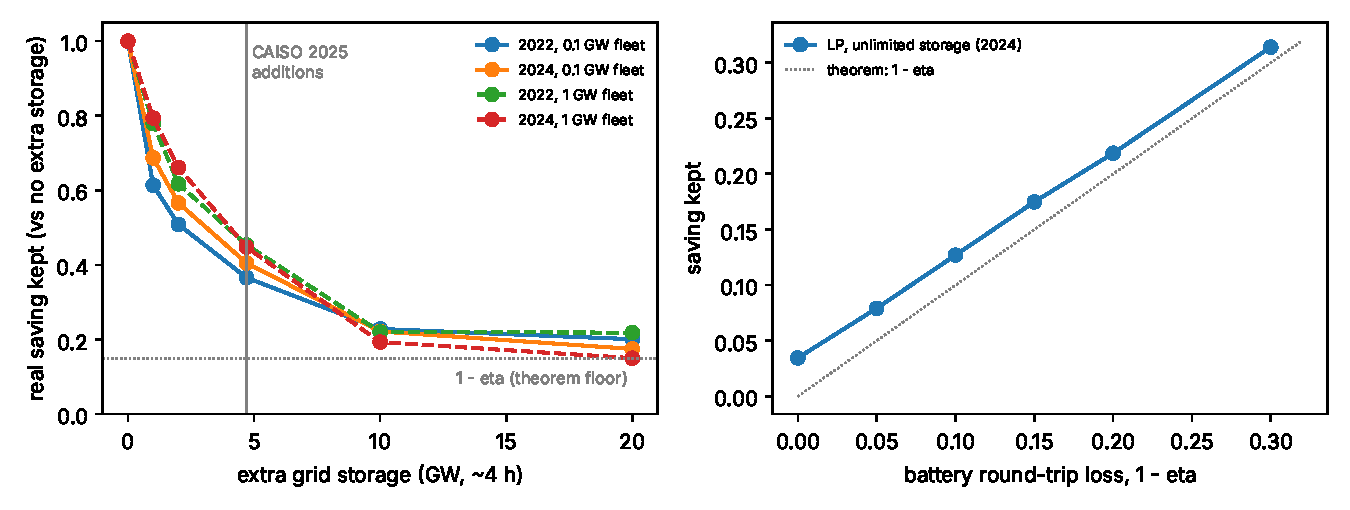
\includegraphics[width=\linewidth]{fig_storage_competition.pdf}
\caption{Left: real saving of carbon-aware shifting kept as extra grid storage is added
(CAISO, $\eta=0.85$). Right: with unlimited storage the saving kept tracks $1-\eta$
(Theorem~\ref{thm:noarb}).}
\label{fig:twobatteries}
\end{figure}
% Numbers: results/storage_competition_*.csv (F32); tests/test_storage_competition.py.

\section{Not Every Knob Is a Battery}
\begin{theorem}[Power-mean law]\label{thm:powermean}
Let a day's work $W=n$ be run at speeds $s_t\ge0$, $\sum_t s_t=n$, with power $s_t^{\alpha}$
($\alpha>1$) and carbon $\sum_t c_t s_t^\alpha$, $c_t>0$. The optimum is
$s_t\propto c_t^{-1/(\alpha-1)}$ and the saving against constant speed is
\[ 1-\frac{\Mp_p(c)}{\Mp_1(c)},\qquad p=-\frac{1}{\alpha-1}, \]
where $\Mp_p(c)=(\frac1n\sum_t c_t^p)^{1/p}$. To second order in the coefficient of variation,
the saving is $\frac{\chi}{2}\mathrm{CV}^2$ with $\chi=\alpha/(\alpha-1)$; as $\alpha\to1$ it tends
to $1-\min_t c_t/\Mp_1(c)$, the deferral optimum.
\end{theorem}
% Empirics (F29): 123 zones x 2020-22, alpha=3: median 0.79% uncapped vs 14.6% for deferral;
% savings scale as CV^1.99 vs CV^1.06.

\section{Related Work}
\textbf{Carbon-aware shifting.} Temporal and spatial shifting were bounded on these traces
by~\cite{sukprasert2024on}; production systems shape load against day-ahead
forecasts~\cite{radovanovic2021carbonaware}; deferral and elasticity were studied
in~\cite{wiesner2021lets,hanafy2024carbonscaler,souza2023ecovisor}, and the choice of average vs
marginal signal in~\cite{sukprasert2024onb,gorka2024electricityemissionsjl}. We add the facility
cap, and with it a closed form.
\textbf{Virtual storage.} Thermostatic and other flexible loads are modelled as virtual batteries
in power systems~\cite{callaway2011achieving,hao2015aggregate}; storage arbitrage can raise
system emissions~\cite{hittinger2015bulk}. Our mapping is exact for deferrable work with a
deadline, and its energy, power and efficiency follow from $(s,\varphi,h)$.
\textbf{Speed scaling.} Energy-optimal speed scaling~\cite{yao1995a} and the carbon/energy
tension of DVFS~\cite{hanafy2023the} motivate Theorem~\ref{thm:powermean}; its second-order form is
a Harberger triangle~\cite{harberger1964the}.
\textbf{Caps on the grid side.} Where the grid itself is under an emissions cap, the avoided
tonnes are moved through the allowance bank unless a supply-adjustment rule absorbs
them~\cite{perino2018new,rosendahl2019eu,perino2019overlapping}; we return to this in
\S\ref{sec:threats}.
% TODO: read the full texts of the virtual-storage and speed-scaling papers.

\section{Threats to Validity}
\label{sec:threats}
\textbf{The grid may be capped.} Every saving in this paper is a change in power-plant
emissions. About 41\% of the cloud-region-weighted shifting saving sits in grids under an
emissions cap (EU ETS, UK ETS, WCI, K-ETS). There, an avoided tonne is real only while a supply
adjustment absorbs it. In the EU this happens while the surplus of allowances (TNAC) is in the
833--1{,}096\,Mt band; it stops within about a year of the market turning short. The saving is
then a fall in the allowance price, not in emissions (the waterbed; companion analysis).
% Average vs marginal signals; fluid work; perfect forecasts (F11 bounds the error);
% assumed alpha for speed scaling; constant gas margin in F24.
\textbf{The grid may already have the battery.} Savings are measured against today's hourly
swing. Where grid storage is growing fast, the counterfactual saving falls towards the
round-trip loss (Section~\ref{sec:twobatteries}); our CAISO counterfactual holds each year's
solar fixed and ignores local congestion, which neither a remote battery nor a remote data
centre can relieve.

\appendix
\section{Proofs}

\begin{proof}[Proof of Theorem~\ref{thm:homog}]
Write the feasible set of \eqref{eq:lp} as $F(\varphi,h)$. Every constraint is linear and its
right-hand side is linear in $(\varphi,h)$: $A_{t-s}=\varphi(t-s)^+$, $A_t=\varphi t$ and
$\varphi+h$. Hence $y\in F(\varphi,h)\iff\lambda y\in F(\lambda\varphi,\lambda h)$. The baseline
$y_t=\varphi$ scales the same way, and the objective is linear, so
$\sum_t c_t(\lambda\varphi-\lambda y_t)=\lambda\sum_t c_t(\varphi-y_t)$; taking the maximum over
the feasible set gives $S(\lambda\varphi,\lambda h)=\lambda S(\varphi,h)$. With
$\lambda=1/\varphi$, $S(\varphi,h)/S(\varphi,\infty)=S(1,h/\varphi)/S(1,\infty)$.
\end{proof}

\begin{proof}[Proof of Proposition~\ref{prop:sinc}]
With one-day windows the problem separates by day. Within a day the work $24\varphi$ must be
placed under the rate bound $\varphi+h$; by the exchange argument (moving work from a dirtier
to a cleaner hour with spare rate never raises cost) the optimum fills the cleanest hours at the
full rate, i.e.\ the sublevel set $\{c_t\le w\}$ of measure $24q$, $q=\varphi/(\varphi+h)$ (the
water level $w$). In the continuum limit for $c(\theta)=\bar c-A\cos\theta$ the sublevel set is
$|\theta|\le\pi q$ and the mean of $c$ on it is
$\bar c-\frac{A}{2\pi q}\int_{-\pi q}^{\pi q}\cos\theta\,d\theta=\bar c-A\sinc(\pi q)$. The served
work $24\varphi$ thus pays $\bar c-A\sinc(\pi q)$ instead of $\bar c$, so
$S=\varphi A\sinc(\pi q)$ per hour of mean load. As $h\to\infty$, $q\to0$ and $S\to\varphi A$; the
uncapped optimum serves the 24 arrivals of a window plus the one arriving at its start,
i.e.\ $25\varphi$ in the cleanest hour, so the peak draw is $1-\varphi+25\varphi=1+24\varphi$.
\end{proof}

\begin{proof}[Proof of Theorem~\ref{thm:battery}]
$Y_t\le A_t\iff B_t\ge0$. With constant arrivals, $Y_t\ge A_{t-s}\iff B_t\le A_t-A_{t-s}=s\varphi$
(for $t\ge s$; for $t<s$ the bound $Y_t\ge0$ is implied by $y\ge0$ and is looser than
$B_t\le s\varphi$ only through the start-up boundary). Since $y_t=\varphi-(B_t-B_{t-1})$,
$0\le y_t\le\varphi+h\iff-h\le B_t-B_{t-1}\le\varphi$. The draw is
$1-\varphi+y_t=1-(B_t-B_{t-1})$. A lossless battery with state of charge $B_t$, discharge
$\delta_t=(B_t-B_{t-1})^+\le\varphi$ and charge $(B_{t-1}-B_t)^+\le h$ in front of a unit load
draws exactly this. The only difference from a cyclic battery is the boundary
$B_0=0$ (nothing is owed at the start) and $B_T=0$ (all work done by the end), which changes
the optimum by at most one cycle of the battery, $O(s\varphi\max_t c_t/T)$ per hour.
\end{proof}

\begin{proof}[Proof of Theorem~\ref{thm:powermean}]
The objective is strictly convex and the constraint linear, so the KKT conditions are
sufficient: $\alpha c_t s_t^{\alpha-1}=\mu$, i.e.\ $s_t=k\,c_t^{-q}$ with $q=1/(\alpha-1)$ and
$k=n/\sum_t c_t^{-q}$ (all $s_t>0$, so the bound $s_t\ge0$ is slack). The cost is
$k^\alpha\sum_t c_t^{1-q\alpha}$ and $1-q\alpha=-q$, so it equals
$n^\alpha(\sum_t c_t^{-q})^{1-\alpha}$. With $p=-q$, $\sum_tc_t^{p}=n\Mp_p^p$ and
$p(1-\alpha)=1$, so the cost is $n\,\Mp_p(c)$. Constant speed costs $n\,\Mp_1(c)$, which gives
the saving. Writing $c_t=\bar c(1+\epsilon_t)$ with $\sum\epsilon_t=0$,
$\Mp_p=\bar c\,(1+\frac{p-1}{2}\overline{\epsilon^2}+O(\epsilon^3))$, so the saving is
$\frac{1-p}{2}\mathrm{CV}^2=\frac{\alpha}{2(\alpha-1)}\mathrm{CV}^2$ to second order. As
$\alpha\to1^+$, $p\to-\infty$ and $\Mp_p\to\min_t c_t$.
\end{proof}

\begin{proof}[Proof of Theorem~\ref{thm:noarb}]
Write the dispatch as a linear programme with energy balance in every hour (dual $m_t$),
charge $c_t$, discharge $d_t$ and state of charge $e_t=e_{t-1}+c_t-d_t/\eta$. Since $c_a>0$ and
$c_a$ is below its power limit, its reduced cost is zero: $m_a=\nu_a$, where $\nu_t$ is the
dual of the state-of-charge equation (the shadow value of stored energy). Likewise $d_b>0$ below
its limit gives $m_b=\nu_b/\eta$. If no energy bound binds between $a$ and $b$,
complementary slackness on those bounds makes $\nu_t$ constant from $a$ to $b$, so
$\nu_a=\nu_b$ and $m_a=\eta\,m_b$. A unit of load moved from $b$ to $a$ changes the optimal
emissions by $m_a-m_b=-(1-\eta)m_b$ by the envelope theorem (exactly, for moves small enough
that the basis does not change).
\end{proof}

\bibliographystyle{ACM-Reference-Format}
\bibliography{refs}   % generated by scripts/build_bib.py
\end{document}
